\documentclass[letterpaper,11pt]{article}

% ---------- CHOOSE A FONT ----------
%
\usepackage[protrusion=true,expansion=true]{microtype} % Better typography

%\usepackage{fouriernc}                     % New Century Schoolbook

\usepackage[bitstream-charter]{mathdesign} % Charter BT

%\usepackage{fontspec}
%\setmainfont{Baskerville}					% Baskerville (use xelatex not pdflatex)

%\usepackage[urw-garamond]{mathdesign}      % Garamond
% or
%\usepackage{fbb}

\usepackage{helvet}                        % Helvetica
%\renewcommand*\familydefault{\sfdefault}

%\usepackage{palatino,mathpazo}             % Palatino
%\RequirePackage[scaled=0.92]{helvet}
%\RequirePackage[scaled=1.02]{inconsolata}
%\linespread{1.05}

%\usepackage{libertine}                      % Libertine

% (or leave all commented out for LaTeX default, Computer Modern)
\usepackage[T1]{fontenc}
% -----------------------------------

% --------- MISC FORMATTING ---------
%
\usepackage{setspace}                % needed for doublespacing
\doublespacing                       % doublespaced line spacing
\usepackage{natbib}                  % for our chosen bibliography style
\usepackage{graphicx}                % for importing graphics into figures
\usepackage{float}                   % better control of figure placement
\usepackage{amsmath}                 % better mathematical typesetting
\usepackage{hyperref}                % for clickable URLs and email addresses
\urlstyle{sf}                        % san-serif font for URLs
\usepackage[margin=1.2in]{geometry}  % control page margins
\usepackage[short]{datetime}         % precise date/time stamp on titlepage
\usepackage[labelfont=bf]{caption}   % make caption labels boldface
\usepackage[bottom]{footmisc}		 % footnotes at bottom of page
\setlength{\skip\footins}{10mm}      % obsessing about footnote spacing
\setlength{\parskip}{1ex}            % space between paragraphs
\usepackage{authblk}                 % author and affiliation formatting
\renewcommand\Affilfont{\small}      %
\usepackage{mathtools}               % mathtools and amsmath
\usepackage{lineno}                  % add line numbers to margin
\def\linenumberfont{\normalfont\footnotesize\sffamily}
\setlength\linenumbersep{7mm}
\linenumbers
%
% -----------------------------------

% ------- CUSTOM TITLE FORMAT -------
%
\makeatletter
\renewcommand{\maketitle}{
\begin{flushleft}       % right align
{\LARGE\@title}         % increase the font size of the title
\vspace{20pt}\\         % vertical space between the title and author name
{\large\@author}        % author name
\\\@date                % date
\vspace{20pt}           % vertical space between the author block and abstract
\end{flushleft}
}
%
% -----------------------------------

\newcommand{\degrees}{\ensuremath{^\circ}} % for nice degree symbol
\usepackage{lipsum}                        % dummy text (you can remove this)

%------------------------------------------------------------------------------
%	TITLE & AUTHORS & AFFILIATIONS
%------------------------------------------------------------------------------

\title{This is the title of the manuscript}

\author[1,2,3,*]{Paul L. Gribble}
\author[1,2,4]{Ford Prefect}

\affil[1]{The Brain and Mind Institute, The University of Western Ontario}
\affil[2]{Department of Psychology, The University of Western Ontario}
\affil[3]{Department of Physiology \& Pharmacology, Schulich School of Medicine \& Dentistry}
\affil[4]{Graduate Program in Neuroscience, The University of Western Ontario}

\date{}

\begin{document}

\begin{singlespace}
\nolinenumbers

\maketitle
\thispagestyle{empty}

\hfill

\begin{flushleft}

%------------------------------------------------------------------------------
%	MAILING ADDRESS & CORRESPONDING AUTHOR INFO
%------------------------------------------------------------------------------

\vspace{35mm}
$^{*}$\textbf{Corresponding Author}\\
\vspace{2ex}
Professor Paul Gribble\\
The Brain and Mind Institute, Dept. Psychology\\
1151 Richmond St, NSC Bldg Room 120\\
London, Ontario, Canada N6A 5B7\\
Phone: +1 519.661.2111 ext. 82237\\
Fax: +1 519.661.3613\\
email: \url{paul@gribblelab.org}

%------------------------------------------------------------------------------
%	KEYWORDS
%------------------------------------------------------------------------------

\vfill
\textbf{Keywords}: blah; blah blah; blah blah blah\\

\vspace{3ex}
{\emph{\today, \currenttime}}

\end{flushleft}

\end{singlespace}

%------------------------------------------------------------------------------
%	ABSTRACT
%------------------------------------------------------------------------------

\newpage
\linenumbers

\section*{Abstract}

\lipsum[1]

%------------------------------------------------------------------------------
%	INTRODUCTION
%------------------------------------------------------------------------------

\newpage
\section*{Introduction}

Blah blah blah lots of crazy research has been done on this topic \citep{Mattar:2005}. Blah blah blah lots of crazy research has been done\footnote{ya ya w8ever} on this topic \citep{Mattar:2005}. Blah blah blah lots of crazy research has been done on this topic \citep{Mattar:2005}. \lipsum[1]

\lipsum[1-3]

%------------------------------------------------------------------------------
%	METHODS
%------------------------------------------------------------------------------

\section*{Methods}

\lipsum[1-2] See equation~\ref{eq:line} for some junk.

\begin{equation}
\hat{Y_{i}} = \beta_{0} + \beta_{1} X_{i} + \epsilon_{i}
\label{eq:line}
\end{equation}

Also see Figure~\ref{fig:setupfig} for some other junk.

\lipsum[1-3]

%------------------------------------------------------------------------------
%	RESULTS
%------------------------------------------------------------------------------

\section*{Results}

Table~\ref{tbl:somedata} is totally meaningless.
\lipsum[1-5]

%------------------------------------------------------------------------------
%	DISCUSSION
%------------------------------------------------------------------------------

\section*{Discussion}

\lipsum[1-8]

%------------------------------------------------------------------------------
%	ACKNOWLEDGEMENTS
%------------------------------------------------------------------------------

\newpage
\section*{Acknowledgements}
This research was supported by grants to PLG by the Canadian Institutes of Health Research and the Natural Sciences and Engineering Council of Canada.

%------------------------------------------------------------------------------
%	REFERENCES
%------------------------------------------------------------------------------

\newpage
\nolinenumbers

\bibliographystyle{jneurosci} 
%\bibliographystyle{jneurophysiol}
\bibliography{refs}

%------------------------------------------------------------------------------
%	TABLES
%------------------------------------------------------------------------------

\newpage
\clearpage
\parbox[c][\textheight][s]{\linewidth}{%
\begin{table}[H]
	\centering
	\begin{tabular}{c|c}
		condition &mean\\
		\hline\hline
		A         &10.1\\
		B         &11.0\\
	\end{tabular}
 \caption{Blah blah some data.}
 \label{tbl:somedata}
\end{table}
}

%------------------------------------------------------------------------------
%	FIGURES
%------------------------------------------------------------------------------

\newpage
\clearpage
\parbox[c][\textheight][s]{\linewidth}{%
\begin{figure}[H]
	\centering
    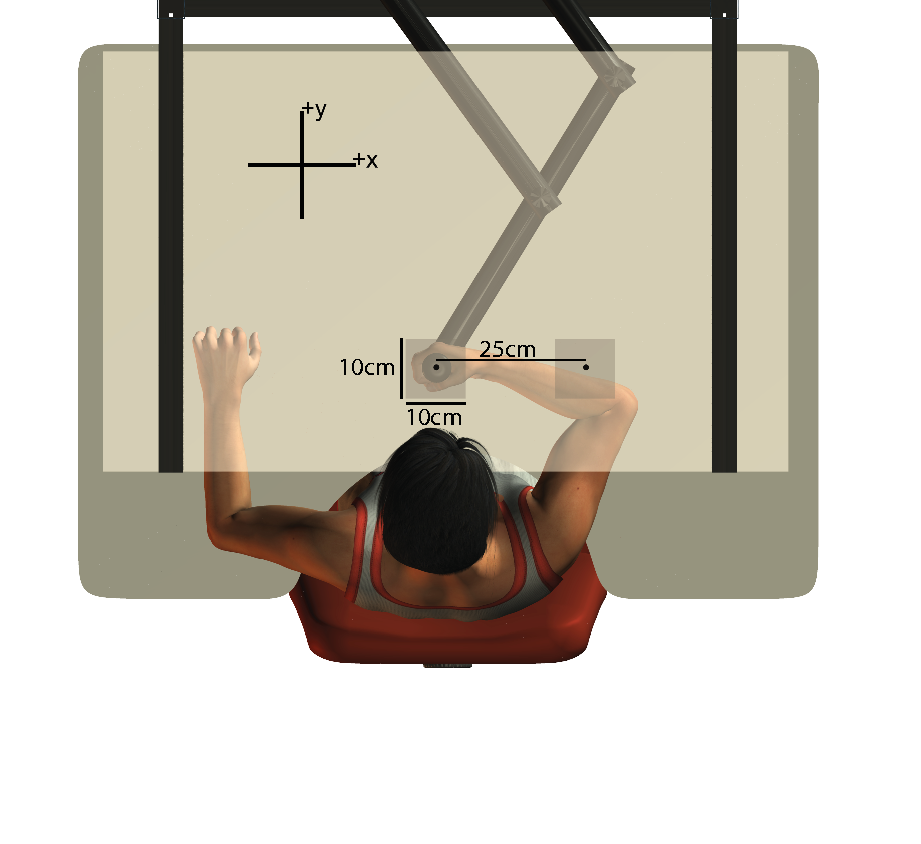
\includegraphics[height=3in]{figure1.pdf}
 \caption{Blah blah blah the robot setup blah.}
 \label{fig:setupfig}
\end{figure}
}

\end{document}

